\chapter{The {\tt Mosaic} Module}\label{ch:mosaic-module}

The \verb#Mosaic# module provides a number of tools for assembling and
generating image mosaics, i.e. large images that are composed of a
number of smaller images.  The applications of this module include
panoramic imaging and aerial/satellite image processing.  There are 
three major facilities provided at this time: compositing many images 
together, using multi-band blending to seamlessly merge overlapping 
images, and generating on-disk image quadtrees to efficiently store 
very large images.

Note that the facilities described in this chapter are currently under
active development, and there may be some API changes in future
releases as new capabilities are added.

\section{{\tt ImageComposite} and Multi-Band Blending}\label{sec:imagecomposite}

The \verb#ImageComposite# template class provides the ability to
composite any number of source images together at arbitrary pixel
offsets.  It was originally designed for assembling tiled panoramas or
aerial/satelite images that have been transformed into a common
coordinate system, though it could be used for many other things as
well.

The main interface is fairly simple.  Just like ordinary Vision
Workbench images, an \verb#ImageComposite# is templatized on its pixel
type.  In most cases you will want to use a pixel type that has an
alpha channel, and if you want to perform image blending then the
pixel type must be floating-point, so the most common pixel type is
\verb#PixelRGBA<float32>#.  You can then configure whether you would 
like to use multi-band blending to merge your images or if you would 
simply like them overlayed by using the \verb#set_draft_mode()# 
method.  It takes a single argument which sould be \verb#true# if 
you simply want to overlay the images and \verb#fales# if you want 
to use the blender.  Blending is a significantly more expensive 
operation.  If your images do not overlap but are simply tiles then 
draft mode is probably what you want. 

Once you have created the composite object, you add source images to
it using the \verb#insert()# method, which takes three arguments: the
image you are adding, and the $x$ and $y$ pixel offset of that image
within the composite.  The \verb#ImageComposite# does not store a copy
of your image.  Instead, it only stores a reference to it in the form
of an \verb#ImageViewRef# object.  This means that you can easily do
things like create a composite of images that could not all fit in
memory simultaneously, e.g. by passing in \verb#DiskImageView#
objects.  Note that only integer pixel offsets are supported: if you
want to shift an image by a fractional amount you will first need to
transform it accordingly.  In most cases you will need to
pre-transform your source images anyway, so this applies no extra
cost.

Once you have added all your images, be sure to call the 
\verb#ImageComposite#'s \verb#prepare()# method.  This method takes 
no arguments, but it does two things.  First, it computes the 
overall bounding box of the images that you have supplied, and 
shifts the coordinate system so that the minimum pixel location 
is $(0,0)$ as usual.  Second, if multi-band blending is enabled, 
it generates a series of mask images that are used by the blender. 
Currently these are saved as files in the current working directory. 
This is admittedly inconvenient behavior and will be changed in a 
future release.

Now that you've assembled and prepared your composite you can use 
it just like an ordinary image, except that per-pixel access is 
not supported.  If the image is reasonably small then you can 
rasterize the entire image by assigning it to an \verb#ImageView#. 
Alternatively, if the composite is huge the usual next step is to 
pass it as the source image to the quad-tree generator, discussed 
in the next section.  You can also use \verb#ImageComposite#'s 
special \verb#generate_patch()# method to manually extract smaller 
regions one at a time.  It takes a single \verb#BBox2i# bounding-box, 
expressed in the re-centered coordinate frame, as its only argument.

Here's a simple example that illustrates how you might blend 
together a number of images on-disk.  It assumes you already know 
the image filenames and their offets within the commposite, and 
that the total composite is small enough to sensible rasterize all 
at once.
\begin{verbatim}
ImageComposite<PixelRGBA<float> > composite;
for( int i=0; i<num_images; ++i ) {
  composite.insert( DiskImageView<PixelRGBA<float> >( image_filename[i] ),
                    image_offset[i].x(), image_offset[i].y() );
}
composite.prepare();
write_image( "composite.png", composite );
\end{verbatim}
For a somewhat more fleshed-out example of how to blend images, 
see the example program \verb#blend.cc# included with the 
\verb#Mosaic# module sources.

\begin{figure}[t]
\centering
  \subfigure[First source]{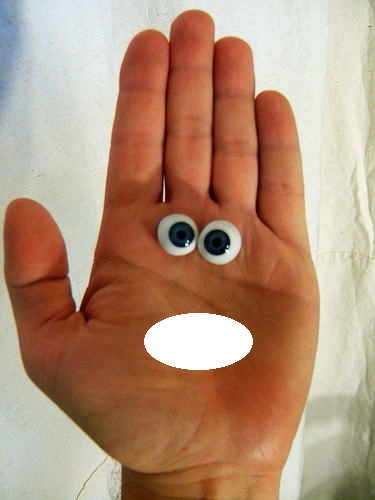
\includegraphics[width=2in]{images/hand.jpg}\label{fig:blend.hand}}
  \hfil
  \subfigure[Second source]{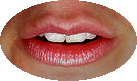
\includegraphics[width=1.23in,trim = -0.25in -1.65in -0.25in 0in]{images/lips.jpg}\label{fig:blend.lips}}
  \hfil
  \subfigure[Blended result]{\includegraphics[width=2in]{images/hand-lips-blend.jpg}\label{fig:blend.result}}
\caption{Example input and output images from the {\tt ImageComposite} multi-band blender.}
\label{fig:blend}
\end{figure}

\section{{\tt QuadTreeGenerator}}\label{sec:quadtreegenerator}

